% !TeX program = pdflatex
% Overleaf main document: quantum_exchange_modulation_paper.tex
% Revised directly from the supplied quantum_exchange_modulation_paper.tex.
% Target: Quantum Information Processing, Regular Article (single-blind review).
% Reviewable revision; see SUBMISSION_README.md before submission.
\documentclass[pdflatex,sn-mathphys-num]{sn-jnl}
\usepackage{amsmath,amssymb,booktabs,tabularx,graphicx,xcolor}
\usepackage{xurl,microtype}
\usepackage[section]{placeins}
\hypersetup{hidelinks}
\setlength{\emergencystretch}{2em}
\newcommand{\Tr}{\operatorname{Tr}}
\newcommand{\D}{\mathcal D}
\newcommand{\E}{\mathbb E}
\newcommand{\sig}{\operatorname{sigmoid}}
% These statements must be supplied by the author, not inferred by the editor.
\newcommand{\FundingStatement}{\textit{Author confirmation required.}}
\newcommand{\CompetingInterestStatement}{\textit{Author confirmation required.}}
\newcommand{\ContributionStatement}{\textit{Author confirmation required.}}
\raggedbottom
\begin{document}
\title[Context-controlled exchange modulation]{Context-controlled exchange modulation for quantum neural networks: physical inductive bias and directional dephasing response}
\author*[1]{\fnm{Dustin} \sur{Keller}}
% Add \email{...} after the author confirms the corresponding address.
\affil*[1]{\orgname{University of Virginia}, \orgaddress{\city{Charlottesville}, \state{Virginia}, \country{USA}}}
% Author to confirm department, postal address, email, and optional ORCID.
% The QIP guideline has conflicting abstract limits; the journal-specific
% 80--100-word instruction is used here. See the readiness note.
\abstract{We introduce context-controlled exchange modulation, a differentiable quantum layer coupling independent preparations through signed partial exchange. On a directional dephasing task, a compact model trained from task-aligned initialization learns an analytic two-copy response across five independently generated physical-axis holdouts. A matched quantum circuit and a 36-feature physics-informed classical regression also recover the target. With 3,840 source copies per query, the learned layer's mean expected inference error is $8.6\times10^{-4}$; direct collective measurement is lower. Reusing Pauli measurements across repeated queries reverses the single-query ranking. The contribution is a physically constrained, trainable representation with explicit access and copy accounting.}
\keywords{Quantum machine learning, quantum data, conditional quantum circuits, partial exchange, dephasing, quantum metrology}
\maketitle

\section{Introduction}
Classical feature-wise linear modulation (FiLM) uses a context network to select affine transformations of hidden features \cite{film}. Quantum data pose a different problem: amplitudes of an unknown state are unavailable as ordinary input features, useful observables need not commute, and a physical channel is linear in its full density-operator input. We consider a source that repeatedly prepares an unknown $m$-qubit state $\rho$, while a classical context $c$ specifies a physical query. A context-controlled quantum layer must identify the registers it consumes, the quantum memory it retains, and the measurements used for prediction.

Partial-SWAP mixing and quantum homogenization are established \cite{ziman,audenaert}. Our construction makes the source rotation and signed exchange into a differentiable, state-valued modulation layer with explicit physical coefficient constraints. Repeated quantum-data interactions also appear in Cha, Park, and Lee's preprint on quantum-data re-uploading \cite{cha_reupload}. Their signal qubit interacts with refreshed input registers; here an equal-size quantum memory receives context-controlled exchange interactions. Related partial-SWAP memory constructions appear in the preprint by Connerty and Evans \cite{connerty_memory}. We make no universality or priority claim for repeated-copy quantum learning.

Conditional parameter generation also predates this work. Haboury et al.'s preprint on emergency escape routing explicitly introduces quantum FiLM for classical graph data \cite{haboury_routing}. Quantum fast-weight programmers use a classical network to update variational-circuit parameters \cite{fastweights}. Lee, Chen, and Tseng program circuit angles and nonlocal observables from each classical input \cite{lee_observables}. Their model uses classical forecasting and reinforcement-learning inputs with no retained quantum-data memory. Our object is a physical map on independent preparations of quantum data, rather than a new name for conditional quantum models.

Quantum convolutional neural networks \cite{qcnn}, learning from quantum experiments \cite{experiments}, quantum-data generalization \cite{generalization}, and shadow-based property prediction \cite{shadows} provide the wider learning setting. Direct multi-copy estimation \cite{ekert} and classical product-feature methods are essential controls for the quadratic response studied here. Their established capabilities motivate an assessment of trainability and physical access costs, rather than a claim of unrestricted quantum advantage.

We distinguish the general streaming network from the compact benchmark. The former composes state-valued layers and has been exercised by a synthetic teacher training fixture. The latter uses one collision, a task-constrained context frame, two output ports, and an affine prediction head. All primary learning-curve numbers refer to this compact model.

\section{Physical layer and quantum-data access}
Let $S$ exchange two complete $d=2^m$ dimensional registers, with $S|i\rangle|j\rangle=|j\rangle|i\rangle$. A classical multilayer perceptron maps context $c$ to rotation angles, an exchange angle $\eta$, and a sign-mixture coordinate $\chi$. The source register is rotated to $\tau_c=V_\phi(c)\rho V_\phi(c)^\dagger$. With $U_\eta=\exp(-i\eta S)$, exact partial tracing gives
\begin{equation}
 \Tr_B[U_\eta(\sigma\otimes\tau_c)U_\eta^\dagger]
 =\cos^2\eta\,\sigma+\sin^2\eta\,\tau_c
 +i\cos\eta\sin\eta[\sigma,\tau_c].\label{eq:swap}
\end{equation}
Choosing $U_\eta$ with probability $\cos^2(\chi/2)$ and $U_{-\eta}$ otherwise yields
\begin{equation}
 \mathcal F_{a,b}(\sigma,\tau_c)=a\sigma+(1-a)\tau_c+ib[\sigma,\tau_c],\quad
 a=\cos^2\eta,\quad b=\tfrac12\sin(2\eta)\cos\chi.
 \label{eq:map}
\end{equation}
The sharp universal physical region is $0\leq a\leq1$ and $b^2\leq a(1-a)$, equivalently the disk $(a-\frac12)^2+b^2\leq\frac14$. Sufficiency follows by choosing $\eta=\arccos\sqrt a$ and $\cos\chi=b/\sqrt{a(1-a)}$ for interior $a$; the endpoints have $b=0$. Necessity follows from positivity: orthogonal pure inputs require $a\in[0,1]$, while pure inputs with squared overlap $q<1$ give $\det\mathcal F_{a,b}=(1-q)[a(1-a)-b^2q]$ in their two-dimensional span. Taking $q\to1$ forces $b^2\leq a(1-a)$. This also applies to self-modulation with unrestricted source rotation. Coherent exchange reaches the boundary, while randomized signs fill the interior. The sign of the commutator follows $U_\eta=e^{-i\eta S}$. Each physical shot uses one chosen sign and one prepared pair. Averaging exact simulator branches adds no copy cost.

For self-modulation, $\sigma=\rho$ and $\tau_c$ is produced from an independent second preparation of $\rho$. The dependence on a single state description is quadratic because the joint input is $\rho\otimes\rho$; no unknown state is cloned and the circuit remains linear in its actual two-register input. If $F_\mu$ denotes an operator feature, then $h_\mu'=\Tr[F_\mu\mathcal F_{a,b}]$ contains the commutator feature $ib\Tr(F_\mu[\sigma,\tau_c])$. For qubits, $\sigma=(I+\mathbf r\cdot\boldsymbol\sigma)/2$ and $\tau_c=(I+\mathbf t\cdot\boldsymbol\sigma)/2$ give $\mathbf r'=a\mathbf r+(1-a)\mathbf t-b\mathbf r\times\mathbf t$: the modulation mixes operator coordinates rather than merely scaling each one.

The generic conditioner is an affine map from $q$ inputs to 16 hidden units, followed by $\tanh$ and an affine map to $p+2$ outputs, where $p=3m+\max(m-1,0)$:
\begin{equation}
 g_\phi(c)=W_2\tanh(W_1c+d_1)+d_2\in\mathbb R^{p+2}.
\end{equation}
The first $p$ outputs give rotation angles $\pi\tanh g_j$; the last two give $\eta=(\pi/2)\sig(g_{p+1})$ and $\chi=\pi\sig(g_{p+2})$. It controls Euler rotations on all source qubits, nearest-neighbor $ZZ$ rotations, $\eta$, and $\chi$. A memory $\omega_0=\rho$ composes through $\omega_{\ell+1}=\mathcal F_{a_\ell,b_\ell}(\omega_\ell,V_\ell(c)\rho V_\ell(c)^\dagger)$. Depth $L$ consumes $L+1$ independent source preparations per execution while retaining at most two data registers at a collision. Measuring selected final Pauli observables and passing their expectations to an affine Torch head makes a scalar predictor. The supplied two-layer trainer verifies differentiable composition, validation selection, and exact checkpoint reload on a synthetic teacher fixture; it is not a physical learning advantage experiment.

\begin{figure}[t]
\centering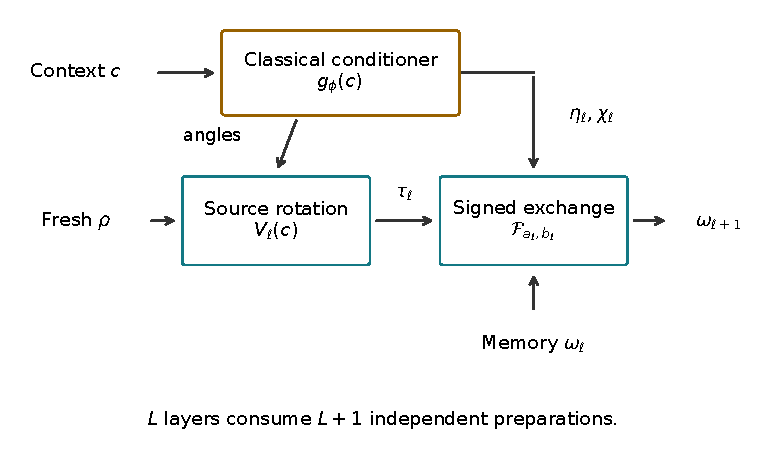
\includegraphics[width=0.94\linewidth]{Fig1.pdf}
\caption{One layer of the general state-valued streaming architecture. A classical context conditioner selects quantum gates; each layer interacts with a fresh source copy and retains quantum memory. The measured terminal observables feed a classical prediction head. The compact benchmark additionally reads both output ports at its final collision.}\label{fig:architecture}
\end{figure}

For fixed context and an affine expectation readout, a depth-$L$ streaming network has degree at most $L+1$ in the input density matrix. This is a degree bound for the stated readout, not for arbitrary nonlinear postprocessing of estimated expectations. Figure~\ref{fig:architecture} summarizes the streaming interface.

\section{Directional dephasing as a benchmark}
For $P=P^\dagger$, $P^2=I$, consider $\dot\rho=\gamma(P\rho P-\rho)$. Define the nonnegative response
\begin{equation}
 D_P(\rho)=\Tr\rho^2-\Tr(\rho P\rho P)
 =\tfrac12\|[P,\rho]\|_{\rm HS}^2,
 \qquad \frac{d}{dt}\Tr\rho^2=-2\gamma D_P(\rho).
 \label{eq:response}
\end{equation}
The two-qubit task takes $P_c=(\mathbf n\cdot\boldsymbol\sigma)\otimes I$, with $\mathbf n=(\sin\theta\cos\varphi,\sin\theta\sin\varphi,\cos\theta)$. This context identifies a perturbation direction; state-preparation parameters are excluded from predictor inputs. The response depends on global correlations even though $P_c$ acts on one spin.

The analytic one-collision circuit rotates a second copy by $V=\exp(-i\pi P/4)$, uses $\eta=\pi/4$ and $\chi=0$, and jointly measures $P$ on both output ports. If $m=\Tr(P\rho)$, the two means are $z_A=m-D_P/2$ and $z_B=m+D_P/2$. Their difference is exactly $D_P$. For joint signs $s,t\in\{-1,1\}$, $t-s$ is an unbiased two-copy estimator. The same ideal grouped outcome distribution is obtained from the collective observable $K_P=(I-P\otimes P)S$, so this identity alone confers no measurement advantage over direct $K_P$ estimation.

The analytic target is available before training. Learning therefore tests whether optimization recovers a known response within a physical model family. The compact 25-parameter model learns four context-frame scales and offsets, sixteen source-circuit angles, two global exchange coordinates, and three affine-head parameters (Table~\ref{tab:learned}). The measured observables remain the known $P(c)$ on both output registers. Its exchange coordinates are global learned scalars; they are not outputs of the generic nonlinear conditioner. Initial frame slopes are randomized near one and the head near an antisymmetric combination, retaining an additional task-aligned prior.

\begin{table}[t]
\caption{Fixed structure and learned parameters of the compact model. The exact analytic rotation and output difference are not imposed as parameter values.}\label{tab:learned}
\begin{tabularx}{\linewidth}{@{}p{.20\linewidth}X r@{}}\toprule
Component & Fixed structure & Parameters\\\midrule
Context frame & $R_z(s_\varphi\varphi+d_\varphi)R_y(s_\theta\theta+d_\theta)$ and inverse & 4\\
Source circuit & Two repetitions of $YI,ZI,IY,IZ,XX,ZZ,XI,IX$ rotations & 16\\
Exchange & Signed full-register exchange and coefficient map & 2\\
Readout & Known $P(c)$ measured on both ports; affine head & 3\\\bottomrule
\end{tabularx}
\end{table}

The matched 28-parameter quantum neural network (QNN) learns operations on both sides of the same exchange primitive. It retains the frame family and query observables, so it is a less constrained control rather than a fully task-agnostic architecture. The classical Torch FiLM comparator receives Pauli features under exact-expectation fitting; widths 12 and 24 and regularization strengths $10^{-5},10^{-3},10^{-2}$ are selected by validation. A six-coefficient Gram comparator is especially strong. Writing $\rho=\frac14\sum_{a,b\in\{I,X,Y,Z\}}r_{ab}\,\sigma_a\otimes\sigma_b$, set $\mathbf r_b=(r_{Xb},r_{Yb},r_{Zb})^T$ and $G=\sum_b\mathbf r_b\mathbf r_b^T$. Then
\begin{equation}
 D_{P_c}(\rho)=\tfrac12[\Tr G-\mathbf n^TG\mathbf n].\label{eq:gram}
\end{equation}
Its untrained analytic version is an oracle when all required Pauli coefficients are available; a fitted version calibrates six coefficients. Their physical feature acquisition must be charged separately.

\subsection{Product-feature classical comparators}
The implemented product kernel is
\begin{equation}\label{eq:kernel}
 k((r,n),(r',n'))=(1+r^Tr')^2(n^Tn')^2,
\end{equation}
where $r$ contains 15 nonidentity Pauli coordinates. It has degree at most two in $r$ and homogeneous degree two in $n$. Since $n^Tn=1$, the $\Tr G$ term can be multiplied by $n^Tn$; the complete target belongs to this feature space. A degree-two polynomial kernel on the concatenation $(r,n)$ would omit the necessary degree-four cross terms, but that is not the implemented kernel. Its poor test performance cannot be attributed to that expressivity restriction.

Three explicit classical feature spaces are fixed for the new comparison: the full 816-dimensional map of Eq.~\eqref{eq:kernel}; 144 products $r_{ib}r_{jb}n_kn_l$ with $i\leq j$, $k\leq l$, and $b\in\{I,X,Y,Z\}$; and 36 products $G_{ij}n_kn_l$. All regression coefficients are fitted by least squares to training labels. The smaller spaces impose known operator-product structure but do not insert the target coefficients. These are physics-informed comparators, not generic neural networks. At the 64-state budget each new 816-feature training matrix has at most rank 320, whereas the 144- and 36-feature matrices have full column rank. Representability alone does not ensure recovery from finite examples.

\section{Experimental protocol and results}
The response is unchanged by reversal of the physical axis: $D_{\mathbf n}=D_{-\mathbf n}$. The original $n_x>0.55$ cap therefore tested oriented directions but did not separate the corresponding physical axes; nine of its 18 training contexts were in the antipodal negative cap. We retain those records as historical development evidence. The new study reserves both caps $|n_x|>0.55$ for axis-only and joint tests, while training and validation use $|n_x|\leq0.55$. There are no duplicate physical states or exact antipodal context pairs across the splits. Nearest axes are audited by $\arccos|\mathbf n\cdot\mathbf n'|$.

One fresh development dataset fixes feature choices and classical hyperparameters. Five independently generated confirmation datasets use separate random streams for physical states, context pools, row selection, and family-balanced training order. Each dataset has 64 candidate training states, 16 validation states, and 128 new test states drawn from the coupled-spin Gibbs, driven product-mixture, and noisy low-rank families. Nested budgets of 8, 16, 32, and 64 complete source states provide five context labels per state, plus 96 validation labels at every budget. The joint test has four held-out-axis contexts for each of 128 new states (512 pairs). The axis-only test uses the actual training states at each budget and four held-out-axis contexts per state. State-only tests use new states with training-region axes. Methods share each dataset and split. Three optimizer starts (17, 31, 73) are retained for every learned configuration. No historical test labels select the reported models.

The compact exchange and matched QNN are trained with differentiable PennyLane circuits through Torch, exact expectations, and validation-selected L-BFGS checkpoints. Classical controls include a training-mean constant, the historical FiLM, a stacked FiLM with a distinct modulated hidden transform at each depth, and a concatenated-input multilayer perceptron. Their feature families comprise raw Pauli coordinates with signed or even $\mathbf n\mathbf n^T$ context, same-spectator Pauli products with even context, and joint direction--Pauli products passed through nonlinear hidden layers. On development data we search 24 configurations per family over widths 16--64, depths 1--3, tanh/SiLU, Adam step sizes $10^{-4}$--$10^{-2}$, and weight decay $0$--$10^{-2}$. A fixed 500/2,000/5,000-update staged schedule retains 6 then 2 candidates per family. Training-only standardization and validation checkpointing are used throughout. The complete 128-attempt search record and all confirmation starts are retained; no configuration is selected from confirmation test MSE. Explicit 816-, 144-, and 36-feature least-squares spaces are fixed from the earlier mathematical review and fitted only to training labels. The 144- and 36-feature spaces deliberately impose operator-product structure.

\begin{table}[t]
\centering
\caption{Mean joint physical-axis test MSE over five independent datasets and three optimizer starts for learned models. Each budget additionally uses 96 validation labels. The 36-feature regression is fitted to the same training labels and has no optimizer starts. All four budgets were rerun in one protocol.}\label{tab:curve}
\small
\begin{tabular*}{\linewidth}{@{\extracolsep{\fill}}rrrrrr@{}}\toprule
States & Train pairs & Exchange & Matched QNN & Product FiLM & Gram-36\\\midrule
8 & 40 & $1.87\times10^{-6}$ & $1.53\times10^{-6}$ & $8.18\times10^{-2}$ & $1.82\times10^{-27}$\\
16 & 80 & $1.39\times10^{-8}$ & $1.51\times10^{-8}$ & $4.67\times10^{-2}$ & $1.95\times10^{-30}$\\
32 & 160 & $6.07\times10^{-9}$ & $1.04\times10^{-8}$ & $3.19\times10^{-2}$ & $2.41\times10^{-30}$\\
64 & 320 & $1.56\times10^{-9}$ & $1.75\times10^{-8}$ & $1.31\times10^{-2}$ & $1.19\times10^{-30}$\\\bottomrule
\end{tabular*}
\end{table}

\begin{figure}[t]
\centering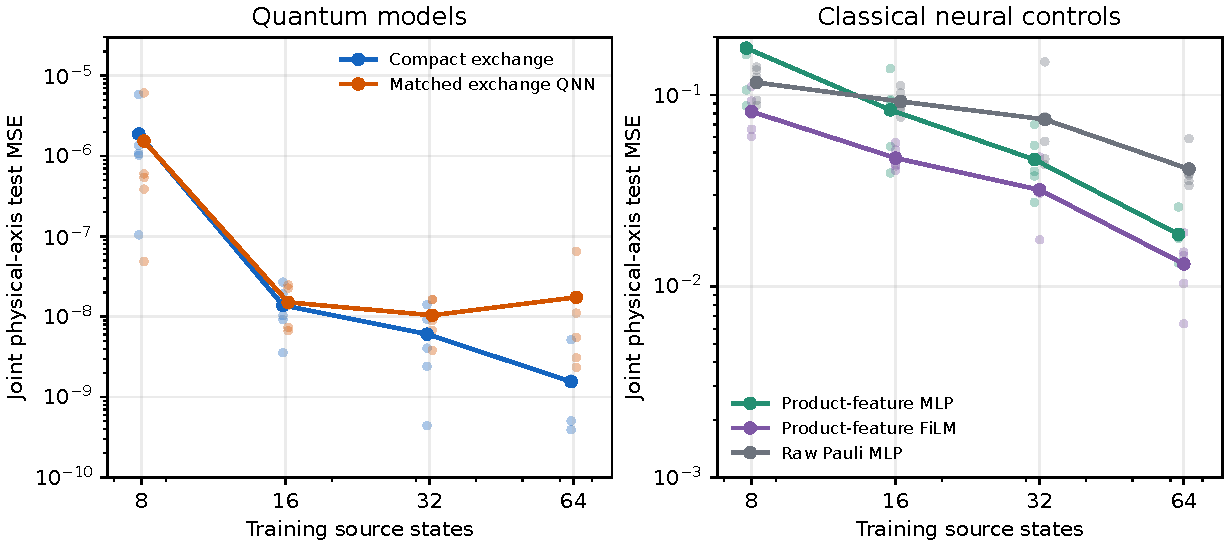
\includegraphics[width=\linewidth]{Fig2.pdf}
\caption{Fresh physical-axis learning curves. Lines give the mean of five dataset means; each translucent point is a dataset mean over three fixed optimizer starts. The product-feature FiLM and multilayer perceptron are development-selected configurations. The exact Gram-36 fit lies below the plotted range and is shown in Table~\ref{tab:curve}.}\label{fig:curve}
\end{figure}

Table~\ref{tab:curve} and Fig.~\ref{fig:curve} show that both two-copy quantum architectures fit the analytic task under the harder physical-axis split. At eight states the matched QNN has slightly lower mean error; at 64 the compact exchange has lower error on four of five datasets. The five 64-state exchange dataset means are $5.06\times10^{-10}$, $3.93\times10^{-10}$, $1.68\times10^{-9}$, $5.18\times10^{-9}$, and $6.60\times10^{-11}$; matched-QNN means are $2.35\times10^{-9}$, $5.55\times10^{-9}$, $6.53\times10^{-8}$, $3.09\times10^{-9}$, and $1.11\times10^{-8}$. These simulator-scale differences are much smaller than inference noise at the copy budgets below. Paired comparisons average repeated queries within each physical source state. State-cluster resampling conditions on the sampled context pool; five dataset outcomes are reported directly rather than treating state--context pairs as independent datasets.

The classical result sharply limits any learning-advantage claim. A fitted 36-feature Gram-product regression recovers every new joint test to numerical precision even at eight states; a fixed analytic exchange circuit with only its three-parameter affine head fitted does so as well. The 144-feature same-spectator map reaches numerical precision from 32 states. By contrast, the unconstrained 816-feature product map has mean joint MSE $0.0357$ at 64 states despite containing the target, because its 320-row training design leaves most coefficient directions unidentified. The mean constant baseline is $0.0571$; the preselected same-spectator FiLM is $0.0131$, and the raw-Pauli multilayer perceptron is $0.0410$. Exact feature access in these training comparisons does not imply zero physical measurement cost. The target is analytically available before learning, so this is a study of physical parameterization, calibration, and inductive bias, not evidence of a general quantum data-efficiency advantage.

\begin{table}[t]
\centering
\caption{Frozen 64-state ablations: mean joint physical-axis test MSE over five datasets and three starts. The neutral initialization changes only the compact model's initial parameters; zero-commutator fixes the signed-exchange mixture at equal weights. The generic 220-parameter source conditioner and its context-blind control retain the known $P(c)$ readout and use their separately development-selected Adam schedule.}\label{tab:ablation}
\small
\begin{tabular*}{\linewidth}{@{\extracolsep{\fill}}lr@{}}\toprule
Model & Mean joint MSE\\\midrule
Compact exchange, aligned initialization & $1.56\times10^{-9}$\\
Matched exchange QNN & $1.75\times10^{-8}$\\
Compact exchange, no commutator & $5.89\times10^{-2}$\\
Compact exchange, neutral initialization & $5.37\times10^{-2}$\\
Generic source conditioner, fixed $P(c)$ readout & $5.47\times10^{-2}$\\
Context-blind source, fixed $P(c)$ readout & $7.02\times10^{-2}$\\\bottomrule
\end{tabular*}
\end{table}

Table~\ref{tab:ablation} isolates parts of the prescribed construction under the frozen schedules. Equal-weight mixing removes its commutator and leaves mean MSE $0.0589$. Neutralizing the context-frame slopes and affine head at initialization raises the mean to $0.0537$, near the constant baseline $0.0571$. Its joint-test median across 15 starts is $1.67\times10^{-6}$: ten starts attain validation MSE below $10^{-4}$, while five fail this descriptive threshold. All 15 task-aligned starts attain it. Thus the neutral mean conceals a mixture of near-solutions and substantial failures; the compact learning result depends on the task-aligned initialization under this optimizer schedule. The generic nonlinear conditioner, with a known $P(c)$ readout but no aligned source circuit, has mean MSE $0.0547$, versus $0.0702$ when its source controller receives a constant context. These outcomes demonstrate optimization sensitivity under these schedules, not a general expressivity separation. The compact model has 25 parameters, the matched QNN 28, and the generic conditioner plus affine head 220. All fits use exact expectations; finite-shot training and device noise remain untested.

\section{Physical applications and limits of transfer}
\textbf{Correlations hidden from marginals.} For $m\ge2$, let $\rho_t=t|\mathrm{GHZ}^+\rangle\langle\mathrm{GHZ}^+|+(1-t)|\mathrm{GHZ}^-\rangle\langle\mathrm{GHZ}^-|$. Every single-qubit marginal is $I/2$, yet $D_{Z_1}(\rho_t)=(2t-1)^2$. The executed Bell ($m=2$) and GHZ ($m=3$) grids each contain 41 mixture weights; prescribed exchange-circuit outputs match independent matrices within $6.67\times10^{-16}$. A model limited to single-qubit marginals cannot resolve the curve. A stronger target-specific comparator measures global $X^{\otimes m}$ parity on two independent copies and multiplies outcomes. With $C$ source copies its variance is $(2-2D^2)/C$, below the exchange estimator's $(4-2D^2)/C$ on this family. This is a correlation representation diagnostic, not trained Bell/GHZ prediction or an exchange shot advantage.

\textbf{Known finite-time law.} The exact dephasing solution gives $\Tr\rho^2-\Tr\rho_T^2=\frac12(1-e^{-4\gamma T})D_P(\rho)$. We select the 64-state compact checkpoint from confirmation dataset 1 by validation MSE among the three fixed starts, then use one prespecified held-out-axis query on each of its 128 new test states. Substitution into the known factor gives 8,064 queries across three rates and 21 times in $[0,3]$. Purity-loss MSE is $6.27\times10^{-13}$ and maximum absolute error is $4.21\times10^{-6}$. The time dependence is supplied by the known law; the network was not trained to discover unknown dynamics.

\textbf{Phase sensitivity.} For the unitary family $\rho_\vartheta=e^{-i\vartheta H}\rho e^{i\vartheta H}$, use the symmetric logarithmic derivative convention $\partial_\vartheta\rho=(L\rho+\rho L)/2$ and quantum Fisher information $F_Q=\Tr(\rho L^2)$. Cerezo et al.'s sub-quantum Fisher information is \cite{cerezo}
\begin{equation}
 \mathcal I_{\rm sub}(\rho,H)
 =4[\Tr(\rho^2H^2)-\Tr(\rho H\rho H)]\leq F_Q(\rho,H).
\end{equation}
Thus $H=P/2$ gives $\mathcal I_{\rm sub}=D_P$, whereas $H=P$ gives $4D_P$. In the first convention, equality holds for pure states and for every qubit state, while mixed multiqubit states can have a strict gap. The executed suite evaluates 261 state-context cases, with independent spectral and symmetric-logarithmic-derivative QFI checks agreeing within $1.95\times10^{-15}$. This applies a known bound rather than introducing one. Figure~\ref{fig:direction} uses the same validation-selected fresh-protocol checkpoint as the finite-time diagnostic and the lowest-ID new test state in confirmation dataset 1. Its $11\times21$ exploratory full-direction grid has MSE $6.05\times10^{-12}$. The grid includes training-region axes and is a one-state illustration, not a population-level holdout test. An uncorrelated spectator can change $D_P$ through purity while leaving the local-generator QFI fixed: for $\rho_A=(I+0.8X)/2$, $P_A=Z$, and $\tau_s=(I+sZ)/2$, $D_{P_A\otimes I}(\rho_A\otimes\tau_s)$ rises from $0.32$ to $0.64$ as $s$ runs from 0 to 1, while $F_Q=0.64$. Thus a noisy estimate of $D_P$ needs an uncertainty allowance before being called a certified numerical lower bound.

\textbf{Thermal spin register.} An exact three-spin diagnostic uses $\rho_\beta=e^{-\beta H}/\Tr e^{-\beta H}$ with $H=-J(Z_1Z_2+Z_2Z_3)-h(X_1+X_2+X_3)-\epsilon(Z_1-Z_3)$, $J=1$, $\epsilon=0.13$, six inverse temperatures from 0 to 4, and 19 fields from 0 to 1.8. Both $X_1$ and $Z_1$ responses are queried on 114 states; global exchange agrees with independent matrices within $7.78\times10^{-16}$. Parallel local partial swaps are a different operation and differ by as much as $0.0970$ on the sampled $\beta=2$ fields. No three-spin model was trained.

\begin{figure}[t]
\centering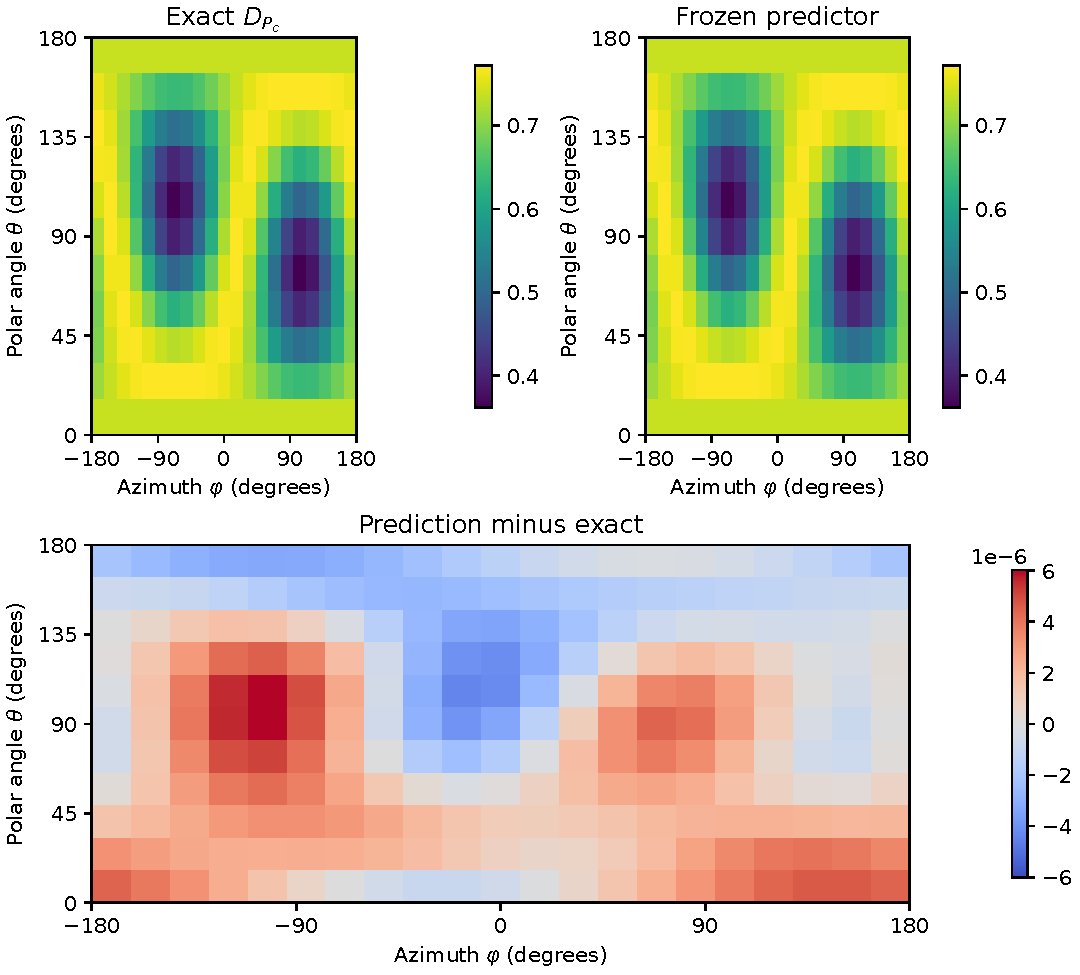
\includegraphics[width=\linewidth]{Fig3.pdf}
\caption{One new test state from confirmation dataset 1, evaluated with its validation-selected 64-state compact checkpoint over an exploratory $11\times21$ full-direction grid. The upper panels show exact response and frozen-model prediction on a common color scale; the lower panel shows prediction error. The panels are regenerated from the new-protocol direction-map CSV. The grid includes training-region axes and is a one-state illustration.}\label{fig:direction}
\end{figure}

\section{Preparation, shots, and logical resources}
Figure~\ref{fig:copies} compares ideal expected inference MSE after exact-expectation training. The benchmark reads both output ports in one execution, consuming two independent source preparations per joint shot. For port weights $w_A,w_B$, means $z_A,z_B$, and joint correlation $q=\E[st]$, its per-shot variance is $w_A^2(1-z_A^2)+w_B^2(1-z_B^2)+2w_Aw_B(q-z_Az_B)$. The last covariance term is retained for every fitted checkpoint. For the analytic difference head, $\operatorname{Var}(\widehat D)=[4(1-m^2)-2D^2]/C$ at $C$ source preparations. Direct $K_P=(I-P\otimes P)S$ has the same entire ideal outcome distribution as the analytic exchange circuit; these are alternative implementations of one observable, not two distinct estimators.

\begin{figure}[t]
\centering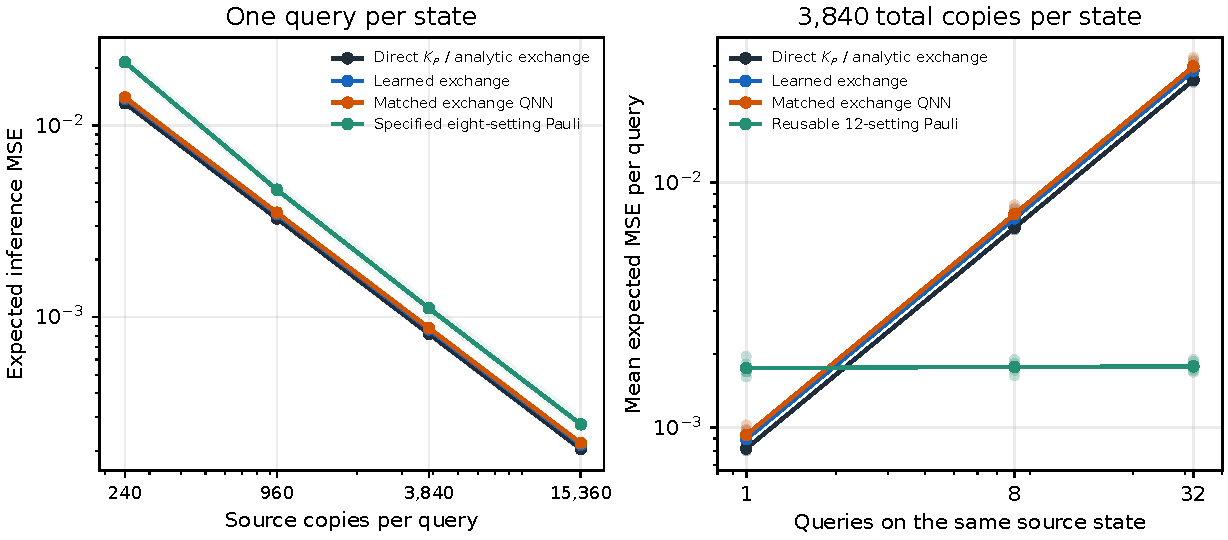
\includegraphics[width=\linewidth]{Fig4.pdf}
\caption{Expected inference MSE on five independent physical-axis test datasets. Left: one query per state at matched source-copy budgets; learned curves average all three optimizer starts at the 64-state training budget, and shaded ranges span dataset means. The green comparator is one specified eight-setting Pauli allocation. Right: 3,840 total source copies per state shared over fresh held-out-axis queries. The prespecified $M=1,8,32$ points are supplemented by exploratory $M=2,3$ crossover checks for direct $K_P$ and reusable Pauli measurements. Quantum shots are divided among queries; a 12-setting unbiased Pauli product estimator reuses its measured features. Quantum checkpoints are selected by validation and classical product risk is estimated with 512 Monte Carlo replicates. These are inference-only ideal measurement laws.}\label{fig:copies}
\end{figure}

At $C=3{,}840$ copies for each single query, the five-dataset mean expected MSE is $8.63\times10^{-4}$ for compact exchange and $8.78\times10^{-4}$ for the matched QNN, averaging all optimizer starts. Analytic exchange/direct $K_P$ gives $8.19\times10^{-4}$, and the specified target-aware eight-setting Pauli allocation gives $1.11\times10^{-3}$. The learned circuits beat this particular Pauli allocation but not direct $K_P$. These values include squared prediction bias and exact joint-port variance. For the compact fit, mean squared bias is only $1.56\times10^{-9}$; its $8.63\times10^{-4}$ error is almost entirely measurement variance. Learned parameters can nearly match the analytic mean response while producing a different two-port outcome law and head weights, hence larger shot variance than the analytic circuit. The Pauli row is neither an optimal classical strategy nor a lower bound; measurement grouping, adaptive allocation, and shadow methods can change its cost \cite{shadows}.

Repeated queries change the accounting. With $3{,}840$ total copies available for each state, $M$ context-specific exchange queries receive $3{,}840/M$ copies each. An independent 12-setting Pauli data collection receives 320 shots per setting once per state; unbiased same-setting square estimators and independent-setting cross products yield a response estimate for every context from those reused outcomes. New nested sets of 1, 8, and 32 held-out-axis queries were fixed without examining target labels. Across five datasets, direct $K_P$ mean expected error per query is $8.20\times10^{-4}$, $6.55\times10^{-3}$, and $2.63\times10^{-2}$ respectively. The reusable Pauli estimator gives approximately $1.75\times10^{-3}$, $1.77\times10^{-3}$, and $1.78\times10^{-3}$, estimated with 512 full-state Monte Carlo replicates per dataset. An additional exploratory check on the first two and three axes of the same frozen query pools places the integer crossover between $M=2$ and $M=3$: mean direct and reusable risks are $(1.64,1.74)\times10^{-3}$ at two queries and $(2.46,1.76)\times10^{-3}$ at three. This reversal compares a context-specific measurement with a reuse-aware measurement and depends on the stated access and allocation rules. Reusing measurements creates correlated errors across a state's queries, which are averaged at the state level rather than treated as independent observations. Classical measurement settings may be grouped more efficiently; no finite-shot training or hardware-noise claim follows from this study.

Logical resources also depend on architecture. A depth-$L$ streaming execution initialized by $\rho$ uses $L+1$ preparations; $N$ shots in each of $s$ separately measured settings use $(L+1)Ns$ preparations. Full-register exchange is $e^{-i\eta S_{AB}}$, not $\prod_j e^{-i\eta S_{A_jB_j}}$. The verified two-qubit-register controlled construction uses four Fredkin gates (32 CNOTs under the specified decomposition), and four additional weight-two Pauli rotations yield a 40-CNOT upper construction. These counts exclude source preparation, routing, compilation, validation labels, gradients, error correction, and device noise. They cannot be used as a complete training or hardware resource comparison.

\section{Discussion}
Context-controlled exchange provides a differentiable physical representation of a two-copy response, with a sharp allowed coefficient region and explicit source-state access. A compact parameterization learns the dephasing functional on independent physical-axis holdouts, while a matched exchange QNN and an analytic three-parameter head calibration also recover it. The 36-feature Gram regression succeeds with only eight training states. These controls locate the contribution in the physical layer, its trainable realization, and transparent copy accounting. They do not support a broad quantum learning or measurement advantage for this analytically known target.

The axis-aware rerun resolves the historical antipodal-support issue. Multiple datasets and state-level paired analyses expose variation hidden by one fixed dataset. The generic conditioner, neutral initialization, context-blind control, and zero-commutator readout probe which prescribed structure matters; their scope is the stated affine port-head benchmark. Further physical tasks with labels from independent dynamics solvers, finite-shot training, grouped or adaptive measurements, and compiled noisy hardware are needed to assess transfer beyond this calibration setting.

\section{Reproducibility}
The historical research implementation and results are preserved at commit \texttt{de6cfa787a13} in \url{https://github.com/zetanaut/quantum-exchange-modulation}. The five-dataset revision, manuscript source, complete numerical records, selected checkpoints, and figure scripts are available under the versioned tag \texttt{qip-revision-v1.2} at \url{https://github.com/zetanaut/quantum-exchange-modulation/tree/qip-revision-v1.2}. The revision records the frozen fresh-data protocol, dataset seeds and hashes, every classical and quantum optimizer start, source-state and axis checks, and expected copy-risk calculations. The five independent dataset outcomes and per-start scores are machine readable. Figure~\ref{fig:direction} and the finite-time diagnostic are regenerated from the validation-selected new-protocol checkpoint and their saved numerical records.

An OpenAI coding assistant was used to draft and execute the revision analysis code, generate figures, and suggest manuscript text. All scientific claims require author review against the saved records before submission. The exact-expectation training comparisons do not include the cost of labels, hyperparameter search, or physical gradient estimation.

\backmatter
\section*{Statements and Declarations}
\textbf{Funding.} \FundingStatement

\textbf{Competing interests.} \CompetingInterestStatement

\textbf{Author contributions.} \ContributionStatement

\textbf{Data and code availability.} The datasets, complete training records, selected checkpoints, scripts, and figure inputs for this revision are available in the public repository at \url{https://github.com/zetanaut/quantum-exchange-modulation/tree/qip-revision-v1.2}, under \texttt{results/submission_revision/} and \texttt{paper/qip/}. The historical snapshot is commit \texttt{de6cfa787a13}.

\appendix
\section{Collective response and copy variance}
For the prescribed response circuit, $V_+=e^{-i\pi P/4}$ commutes with $P$ and $\tau_+=V_+\rho V_+^\dagger$. The two reduced output means are $z_A=m-D_P/2$ and $z_B=m+D_P/2$, and the joint correlation is $\langle P_A P_B\rangle=m^2$. Thus
\begin{equation}
 \Pr(s,t)=\tfrac14(1+s z_A+t z_B+st\,m^2),\qquad
 \operatorname{Var}\!\left[\frac1N\sum_{j=1}^N(t_j-s_j)\right]
 =\frac{2(1-m^2)-D_P^2}{N}.
\end{equation}
For $C=2N$ source preparations this reduces to the copy-normalized variance reported in the main text. More strongly, if $W=U_{\pi/4}(I\otimes V_+)$, then $W^\dagger(P_B-P_A)W=(I-P\otimes P)S=K_P$. Hence the grouped terminal outcomes have the same entire ideal spectral distribution as direct $K_P$ measurement, not only its mean. This establishes the strongest analytic collective-observable control for the specified query.

% The sn-jnl class selects sn-mathphys-num.bst; keep that file and references.bib beside this main .tex.
\typeout{QIP bibliography boundary for BibTeX}
\bibliography{references}
\end{document}
